%\documentclass[11pt]{article}
\documentclass{elsart}

\usepackage{gpeyre}

\usepackage{epsfig}
\usepackage{epstopdf}

\newcommand{\zun}{[0,1]}
\newcommand{\zd}{[0,1]^d}
\newcommand{\fe}{f}

%\psdraft

% format A4
%\usepackage{vmargin}
%\setpapersize{A4}

% FORMAT double interligne
%\renewcommand{\baselinestretch}{2}

\newcommand{\myparagraph}[1]{ \vspace{2mm}\noindent\textbf{#1} \: }
\newcommand{\Proj}{\text{Proj}}


\graphicspath{{./images/}}


\begin{document}

\begin{frontmatter}

\title{Manifold Models for Signals and Images}


\author{Gabriel Peyr\'e\corauthref{cor1}} %\thanksref{label2}}



\ead{gabriel.peyre@ceremade.dauphine.fr}
\ead[url]{http://www.ceremade.dauphine.fr/}
% \thanks[label2]{}
\corauth[cor1]{Place du Mar\'echal De Lattre De Tassigny, 75775 Paris Cedex 16, France}
\address{CNRS and CEREMADE, Universit\'e Paris-Dauphine} %\thanksref{label3}

% \maketitle


\begin{abstract}
	This article proposes a new class of models for natural signals and images. These models constrain the set of patches extracted from the data to analyze to be close to a low dimensional manifold. This manifold structure is detailed for various ensembles suitable for natural signals, images and textures modeling. These manifolds provide a low-dimensional parameterization of the local geometry of these datasets. These manifold models can be used to regularize inverse problems in signal and image processing. The restored signal is represented as a smooth curve or surface traced on the manifold that matches the forward measurements. A manifold pursuit algorithm computes iteratively a solution of the manifold regularization problem. Numerical simulations on inpainting and compressive sensing inversion show that manifolds models bring an improvement for the recovery of data with geometrical features.
	% In the discrete setting, the manifold can be either known analytically or estimated from exemplars using a graph structure.
\end{abstract}

\begin{keyword}
% keywords here, in the form: keyword \sep keyword
signal processing \sep image modeling \sep texture \sep manifold.
% PACS codes here, in the form: \PACS code \sep code
\PACS code \sep code
\end{keyword}
\end{frontmatter}

%\begin{AMS}
%41A25, 42C40, 65T60
%\end{AMS}



%%%%%%%%%%%%%%%%%%%%%%%%%%%%%%%%%%%%%%%%%%%%%%%%%%%%%%%%%%%%%%
%%%%%%%%%%%%%%%%%%%%%%%%%%%%%%%%%%%%%%%%%%%%%%%%%%%%%%%%%%%%%%
%%%%%%%%%%%%%%%%%%%%%%%%%%%%%%%%%%%%%%%%%%%%%%%%%%%%%%%%%%%%%%
%		Introduction
%%%%%%%%%%%%%%%%%%%%%%%%%%%%%%%%%%%%%%%%%%%%%%%%%%%%%%%%%%%%%%
%%%%%%%%%%%%%%%%%%%%%%%%%%%%%%%%%%%%%%%%%%%%%%%%%%%%%%%%%%%%%%
%%%%%%%%%%%%%%%%%%%%%%%%%%%%%%%%%%%%%%%%%%%%%%%%%%%%%%%%%%%%%%


Modeling the geometry of signals and images is at the core of recent advances in sound and natural image processing. Edges and texture patterns create complex non-local interactions that must be captured to improve denoising and inverse problem resolution. This paper studies these geometries for several sounds, images and textures models. The set of local patches in the dataset is modeled using smooth manifolds. These local features trace a continuous curve (resp. surface) on the manifold, which is a prior that is used to solve inverse problems.


%%%%%%%%%%%%%%%%%%%%%%%%%%%%%%%%%%%%%%%%%%%%%%%%%%%%%%%%%%%%%%
%%%%%%%%%%%%%%%%%%%%%%%%%%%%%%%%%%%%%%%%%%%%%%%%%%%%%%%%%%%%%%
%%%%%%%%%%%%%%%%%%%%%%%%%%%%%%%%%%%%%%%%%%%%%%%%%%%%%%%%%%%%%%
\section{Introduction}

%%%%%%%%%%%%%%%%%%%%%%%%%%%%%%%%%%%%%%%%%%%%%%%%%%%%%%%%%%%%%%
\subsection{Previous Works}

\myparagraph{Global manifold models for image libraries.}
Dimensionality reduction methods such as Isomap \cite{tenenbaum-isomap}, eigenmaps \cite{belkin-laplacian-eigenmaps}, LLE \cite{roweis-lle} or diffusion geometries \cite{coifman-geometric-diffusion} have been used to study the manifold structure of a library of images. The manifold regularity of certain images ensembles is emphasized by Donoho and Grimes \cite{donoho-isomap} and Wakin et al. \cite{wakin-multiscale-structure}. These global non-linenar models have applications to image synthesis in computer vision \cite{aharon-lips}.  Manifold valued functions are introduced in \cite{ur-uaman-multiscale-manifold} and can be processed using multiscale methods. A global manifold model is used by Baraniuk and Wakin \cite{wakin-random-proj-manifold} to reconstruct an image from compressive sensing measurements. 

\myparagraph{Local edge manifold and cartoon images.}
The study of sets of patches of $3 \times 3$ pixels extracted from natural images has been carried over by Lee et al. \cite{lee-non-linear-stats}. They report statistical evidences showing that the set of high contrast patches is located around the manifold of edges. These results have been refined by Carlsson et al. \cite{carlsson-local-behavior} who perform a simplicial approximation of the manifold. 

Manifold parameterizations of local structures such as edges and corners is used in computer vision to detect salient features in images. Baker et al. \cite{baker-parametric}  propose fast algorithms to search in a feature manifold. Huggins and Zucker \cite{huggins-local-pca} propose a local principal components analysis over a feature manifold to speed up computations. 

Images with contours contain sharp variations along regular curves that make wavelets sub-optimal because of their square support \cite{mallat-book}.  Total variation methods \cite{rudin-tv} cannot make use of the regularity of the edge curves since they only constraint the overall length of the edges. A simple image model to describe geometric images is the cartoon model introduced by Donoho \cite{donoho-wedglets}. A cartoon function is regular outside a set of edge curves which are themselves regular. Several tools from harmonic analysis give optimal representations for such cartoon functions, including wedgelets \cite{donoho-wedglets}, curvelets \cite{candes-tight-frame} and bandlets \cite{bandelets-siam,bandelets-peyre}.

Cartoon images and the edge manifold is studied in Section \ref{sec-manifold-cartoon-images}.

\myparagraph{Locally parallel textures.}
Some natural textures are composed of nearly parallel stripes that are modeled as local oscillations. This model of locally parallel textures is the extension to images of the model of locally stationary sounds. This model is studied Ben-Shahar and Zucker \cite{ben-shahar-perceptual} who emphasis the role of the regularity of the underlying flow in image perception. Spatially varying orientations has been used in psychophysics as the simplest model for geometric textures, see for instance the model of second order edges of Landy and co-workers \cite{landy-2nd-order}.

Demanet and Ying \cite{demanet-waveatoms} propose a waveatom basis to capture efficiently the anisotropic regularity of such textures. Adaptive decompositions such as the grouplets bases of Mallat \cite{mallat-grouplets} capture efficiently turbulent textures. The idea of characterizing textures as highly oscillating functions  has been introduced by Meyer \cite{meyer-oscillating}. Efficient algorithms to separate such textures from a cartoon sketch have been proposed by Aujol et al. \cite{aujol-decomposition} among others.

Section \ref{sec-manifold-oscillation-1d} studies locally parallel textures and shows how a patch manifold can be optimized to capture specific texture patterns.

\myparagraph{Non-local and sparse patch processing.}
The most successful texture synthesis algorithms perform a consistent recopy of pixels and patches \cite{efros-nonparam-sampling,wei-texture-synthesis}. Local manifolds of patches have been used for texture synthesis and modification \cite{wang-appearance,matusik-texture-design}.  Non-local filtering based on patch comparison has be proposed by Buades et al. \cite{buades-nl-means} to perform denoising, and adapted orthogonal basis can be constructed from non-local graphs \cite{peyre-manifold-bases}. Non local regularization is able to solve inverse problems such as super-resolution \cite{protter-nl-superesol}�or compressive sensing \cite{peyre-nonlocal-ip}

Wavelets and more recent tools from harmonic analysis \cite{mallat-book} leads to efficient image compression, but fail to capture the geometry of natural images and textures \cite{simoncelli-natural}. The weakness of fixed representations can be alleviated by learning a dictionary from examples. Olshausen and Field \cite{olshausen-simple-cell} obtained an optimized set of oriented filters trained on patches extracted from natural images. Other algorithms have been proposed that minimizes various sparsity enforcing criterions, see for instance \cite{engan-mod,delgado-dictionary-learning,lewicki-learning-overcomplete,aharon-ksvd}. These dictionaries on small patches can be used to perform image denoising \cite{elad-aharon-denoise}, facial image compression \cite{bryt-facial-ksvd} and to solve inverse problems such as inpainting \cite{mairal-color} or image separation \cite{peyre-learning-dico}.

Section \ref{subsec-sparse-patches} details a sparse model for patches originally introduced by Peyr\'e \cite{peyre-sparse-textures} for texture synthesis. It fits into our patch manifold framework, and can thus be used to regularize inverse problems, as shown in Section \ref{sec-inverse-pbm}.


%%%%%%%%%%%%%%%%%%%%%%%%%%%%%%%%%%%%%%%%%%%%%%%%%%%%%%%%%%%%%%
\subsection{Contributions}

Section \ref{sec-example-manifold} details several patch manifolds for signals and images. This extends previous studies that consider mainly local edge models and makes the connection with non-local filtering and sparse patch decompositions. 

Section \ref{sec-inverse-pbm} proposes a manifold regularization to solve inverse problems, which relies on the local manifold structure of images. Numerical results are shown on inpainting and compressive sensing reconstruction. This extends global manifold regularization that works for library of images and regularization with sparsity prior in patch dictionaries.


%%%%%%%%%%%%%%%%%%%%%%%%%%%%%%%%%%%%%%%%%%%%%%%%%%%%%%%%%%%%%%
%%%%%%%%%%%%%%%%%%%%%%%%%%%%%%%%%%%%%%%%%%%%%%%%%%%%%%%%%%%%%%
%%%%%%%%%%%%%%%%%%%%%%%%%%%%%%%%%%%%%%%%%%%%%%%%%%%%%%%%%%%%%%
%		Introduction
%%%%%%%%%%%%%%%%%%%%%%%%%%%%%%%%%%%%%%%%%%%%%%%%%%%%%%%%%%%%%%
%%%%%%%%%%%%%%%%%%%%%%%%%%%%%%%%%%%%%%%%%%%%%%%%%%%%%%%%%%%%%%
%%%%%%%%%%%%%%%%%%%%%%%%%%%%%%%%%%%%%%%%%%%%%%%%%%%%%%%%%%%%%%
\section{Manifolds of Signals and Images Patches}

%%%%%%%%%%%%%%%%%%%%%%%%%%%%%%%%%%%%%%%%%%%%%%%%%%%%%%%%%%%%%%
\subsection{Local Manifold Model for Patches}

A patch $p_x(f)$ of width $\tau>0$ extracted from a signal ($d=1$) or image (d=2) $f \in \Ldeux([0,1]^d)$ around $x \in [0,1]^d$ is 
\begin{equation}
		\label{eq-defn-patch}
		\foralls t \in [-\tau/2,\tau/2]^d, \qquad p_x(f)(t) = f(x+t). 
\end{equation}
The point $x$ is the center of the patch $p_x(f)$ and the width $\tau$ controls the size of typical features to analyze. 


A signal ensemble $\Theta \subset \Ldeux([0,1]^d)$ gathers typical data one is interested in. The patch manifold associated to this ensemble is
\begin{equation}
	\label{eq-defn-patch-ensemble}
	\Mm = \enscond{p_x(g) }{x \in [0,1]^d, g \in \Theta} \subset \Ldeux([-\tau/2,\tau/2]^d).
\end{equation}
Section \ref{sec-example-manifold} details the structure of $\Mm$ for various signal and image ensembles $\Theta$. Section \ref{sec-inverse-pbm} uses a fixed manifold $\Mm$ to regularize inverse problems. 

Figure \ref{fig-manifold-examples} shows two examples of image and texture ensembles $\Th$. The patches extracted from these images are parameterized by a small number of variables (for instance the direction of the edge, the orientation and frequency of the texture) so that the set $\Mm$ has the structure of a smooth manifold.


\myfigure{
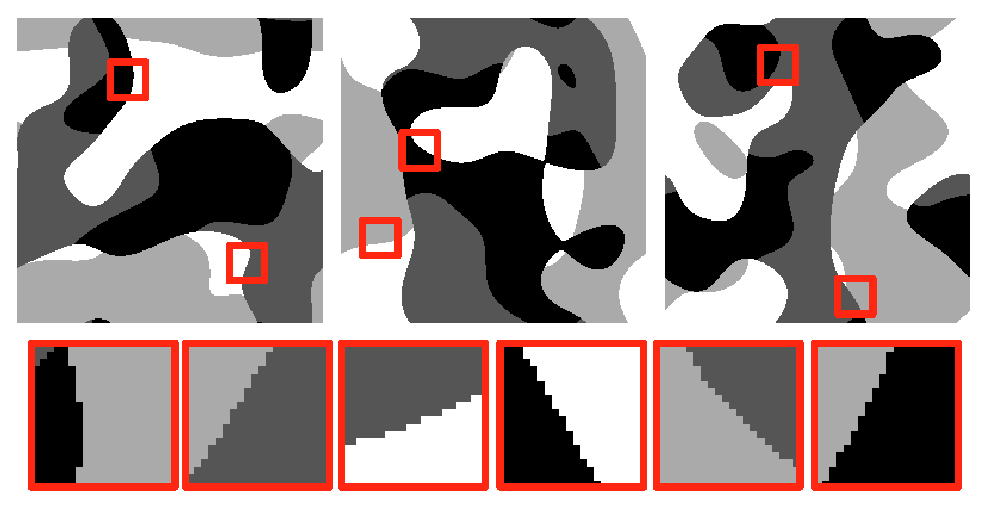
\includegraphics[width=0.48\linewidth]{manifolds-examples/manifold-edges.eps} \hspace{2mm}
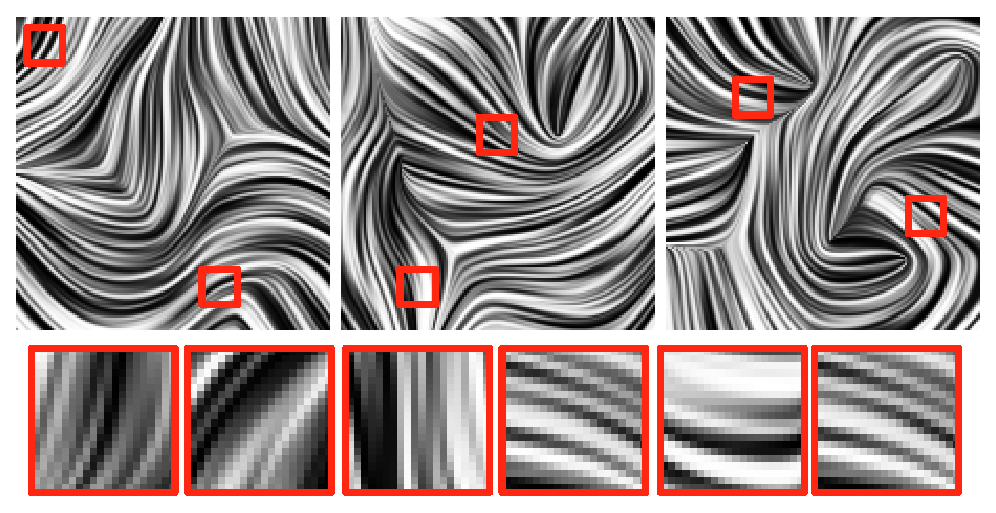
\includegraphics[width=0.48\linewidth]{manifolds-examples/manifold-textures.eps}
}{
Examples of patches $p_x(f) \in \Mm$ extracted from images $f \in \Th$ in 
the cartoon images ensemble (left, see section \ref{sec-manifold-cartoon-images}) and
in the oscillating textures ensemble (right, see section \ref{sec-manifold-locpar-textures}).
%
}{fig-manifold-examples}




%%%%%%%%%%%%%%%%%%%%%%%%%%%%%%%%%%%%%%%%%%%%%%%%%%%%%%%%%%%%%%
\subsection{Manifold Parameterization}

The set $\Mm$ is assumed to have a smooth manifold structure and is thus locally parameterized around a feature $p \in \Mm$ using a smooth mapping
\begin{equation*}
	\phi : \Om \subset \RR^m \longrightarrow \phi(\Om) \subset \Mm,
\end{equation*}
where $p \in \phi(\Om)$. The dimension $m$ gives the number of parameters that describe the local geometry of images in~$\Th$. 

All the manifold studied in the sequel are globally described using a small number $m$ of parameters. A global parameter domain $\Om \subset \RR^{m-k} \times (\Sun)^k$ is used to parameterize the whole manifold. The circle $\Sun = \enscond{\th}{|\th|=1}\simeq [0,2\pi)$ is used to account for directional features and can be replaced occasionally by the set of orientations $\tSun$ (half circle) .
%\eq{	\tSun = (\Sun / \sim) \simeq [0,\pi) \qqwhereqq
%	\pa{\th \sim \th' \Leftrightarrow \th=\th \text{ mod } \pi}. }

Thanks to this global parameterization, any signal $f \in \Th$ is represented as a curve (for signals when $d=1$) or a surface (for images when $d=2$) traced on the manifold $\Mm$ and equivalently over the parameter domain $\Om$
\eql{\label{eq-defn-curve-manifold}
	\choice{
		c_f : x \mapsto p_x(f) \in \Mm, \\
		\Cc_f : x \mapsto \phi^{-1}(p_x(f)) \subset \Om.
	}
}
For signals (resp. images) with periodic boundary conditions, the corresponding curve (resp. surface) is closed (resp. is topologically equivalent to a torus). 

The mapping $c_f$ is a manifold valued function and in the following $\Vv(\Mm)$ is the set of such functions from $\zd$ to $\Mm$. These functions have been studied in \cite{ur-uaman-multiscale-manifold}.


%%%%%%%%%%%%%%%%%%%%%%%%%%%%%%%%%%%%%%%%%%%%%%%%%%%%%%%%%%%%%%
\subsection{Global Manifold Model for Signals and Images}
\label{subsec-global-manif-model}

The local manifold $\Mm$ introduced in \eqref{eq-defn-patch-ensemble} defines a patch manifold model that assigns to any patch $p \in \Ldeux([-\tau/2,\tau/2]^d)$ its distance to $\Mm$
\eql{
	\label{eq-defn-manifold-proj}
	d(p,\Mm) = \norm{p-\Proj_{\Mm}(p)}
	\qwhereq
	\Proj_{\Mm}(p) = \uargmin{q \in \Mm} \norm{p-q}
}
The goodness of fit $d(p,\Mm)$ to the manifold model is extended to a signal or image $f$ by averaging the distances of all the patches
\eql{\label{eq-defn-energy-manifold}
	E_{\Mm}(f) = \int_{[0,1]^d} d(p_x(f),\Mm)^2 \d x = 
	\int_{[0,1]^d} \norm{ p_x(f) - \Proj_{\Mm}(p_x(f)) }^2 \d x.
}
A signal or an image $f$ with a low energy $E_{\Mm}(f)$ traces a curve (resp. a surfaces) $c_f = \{ p_x(f) \}_{x \in \zd}$ close to the low dimensional manifold $\Mm$. This curve is projected on the manifold $\Mm$ and on the parameter domain $\Om$ as follow
\eql{\label{eq-curve-manifold-projected}
	\tilde c_f(x) =  \Proj_{\Mm}(p_x(f)) \in \Mm
	\qandq
	\tilde \Cc_f(x) = \phi^{-1}(\tilde c_f(x)) \in \Om.
}


The projection $\Proj_{\Mm}(f)$ of a signal $f$ on the patch manifold model generated by $\Mm$ is achieved by computing the set of patches $c_f(x) = p_x(f)$, projecting these patches on the manifold $\tilde c_f(x) =  \Proj_{\Mm}( c_f(x) )$ and then reconstructing a signal $\Proj_{\Mm}(f) = \text{Aver}(\tilde c_f)$ from $\tilde c_f$ using the averaging operator
\eql{\label{eq-averaging} 
	\text{Aver}(c)(x) = 
	\frac{1}{\tau^d} \int_{|x-z| \leq \tau/2} p_z(x-z) \d z
			\qwithq p_z = c(z).
}

Section \ref{sec-example-manifold} studies for several signal and image ensembles $\Th$ the geometry of $\tilde c_f$. Section \ref{sec-inverse-pbm} uses the manifold energy $E_\Mm$ to regularize inverse problems.

%%%%%%%%%%%%%%%%%%%%%%%%%%%%%%%%%%%%%%%%%%%%%%%%%%%%%%%%%%%%%%
%%%%%%%%%%%%%%%%%%%%%%%%%%%%%%%%%%%%%%%%%%%%%%%%%%%%%%%%%%%%%%
%%%%%%%%%%%%%%%%%%%%%%%%%%%%%%%%%%%%%%%%%%%%%%%%%%%%%%%%%%%%%%
%		Examples of Patch Manifolds
%%%%%%%%%%%%%%%%%%%%%%%%%%%%%%%%%%%%%%%%%%%%%%%%%%%%%%%%%%%%%%
%%%%%%%%%%%%%%%%%%%%%%%%%%%%%%%%%%%%%%%%%%%%%%%%%%%%%%%%%%%%%%
%%%%%%%%%%%%%%%%%%%%%%%%%%%%%%%%%%%%%%%%%%%%%%%%%%%%%%%%%%%%%%
\section{Examples of Patch Manifolds}
\label{sec-example-manifold}

This section studies the manifold model introduced in the previous section for various image and signal ensembles $\Th$.

%%%%%%%%%%%%%%%%%%%%%%%%%%%%%%%%%%%%%%%%%%%%%%%%%%%%%%%%%%%%%%
%%%%%%%%%%%%%%%%%%%%%%%%%%%%%%%%%%%%%%%%%%%%%%%%%%%%%%%%%%%%%%
\subsection{Manifold of Smooth Variations}
\label{sec-manifold-smooth-functions}

Smooth signals and images $f$ belongs to the set 
\begin{equation*}
	\Th = \enscond{f \in \Cun(\zd)}{ \norm{f}_{\infty} \leq a_{\max}
	\qandq \bnorm{ \pd{f}{x_i} }_{\infty} \leq b_{\max}}.
\end{equation*}
Patches from functions $f \in \Th$ are well approximated by affine functions
\begin{equation*}
	\foralls |t|\leq \tau/2, \quad p_x(f)(t) \approx a(x) + \dotp{b(x)}{t}
	\qwhereq
	\choice{
	a(x) = f(x), \\
	b(x) = \nabla_x f.
	}
\end{equation*}
This leads us to consider the patch manifold of affine functions
\eql{\label{eq-defn-manifold-smooth-variations}
	\tilde \Mm = \enscond{ p_{a,b} }{ |a|\leq a_{\max} \text{ and } |b_i|\leq b_{\max} },
	\qwhereq
	p_{a,b} : t \mapsto a+\dotp{b}{t}
}
which is close to the true manifold $\Mm$ generated by patches of $\Th$ as defined in \ref{eq-defn-patch-ensemble}. In the following, for simplicity, we do not make the distinction between $\tilde \Mm$ and $\Mm$.

This affine manifold is parameterized globally as follow
\begin{equation*}
	\phi :
	\left\{
	\begin{array}{ccc}
		[-a_{\max},a_{\max}] \times [-b_{\max},b_{\max}]^d & \longrightarrow & \Mm\\
		(a,b) & \longmapsto & \bpa{t \mapsto a + \bdotp{b}{t}}.
	\end{array}
	\right.
\end{equation*}
This shows that $\Mm$ is a flat Euclidean manifold of dimension $d+1$. Geodesic distances along $\Mm$ are equal, up to a constant, to the Euclidean distance over the parameter domain. This analysis can be carried over for functions of higher smoothness or for bandlimited functions. These smooth signals ensembles are processed optimally using linear Fourier decomposition and linear filtering.

% The constants $\al = \tau^{-d/2}$ and $\be = (2\sqrt{3})\tau^{-d/2-1}$ are defined to ensure that $\phi$ is an isometry. 

The projection $\Proj_{\Mm}(p)$ of $p \in \Ldeux([-\tau/2,\tau/2]^d)$ is computed by a linear regression.


%%%%%%%%%%%%%%%%%%%%%%%%%%%%%%%%%%%%%%%%%%%%%%%%%%%%%%%%%%%%%%
\myparagraph{Uniformly regular 1D signals.}
Smooth periodic signals in 1D are locally described using the 2D manifold $\Mm$ of affine 1D functions. Each signal $f$ defines a 1D submanifold $\tilde c_f \subset \Mm$, see equation \eqref{eq-curve-manifold-projected}. This submanifold corresponds to a curve over the parametric domain 
\begin{equation*}
	\foralls x \in \zun, \quad \tilde \Cc_f(x) = \phi^{-1}( \Proj_\Mm(p_x(f)) ) \approx (f(x), f'(x)) \in \RR^2.
\end{equation*}
Figure \ref{fig-smooth-1d-manifold} shows an example of a smooth function $f$ together with the corresponding embedding $\tilde c_f$ in (b). This curve  $\tilde c_f$ exihibits self intersections, which correspond to points $x \neq y$ where $f(x)=f(y)$ and $f'(x)=f'(y)$. 

% On (c) one can see a comparison of the geodesic distance on $\Mm$ and $\tilde c_f$ from some central starting point $x_0$. This shows that $d_{\Mm}(p_{x_0}(f),p_x(f)) \leq d_{\tilde c_f}(p_{x_0}(f),p_x(f))$ since $\tilde c_f$ is proper subset of $\Mm$.

\myfigure{
\begin{tabular}{cc}
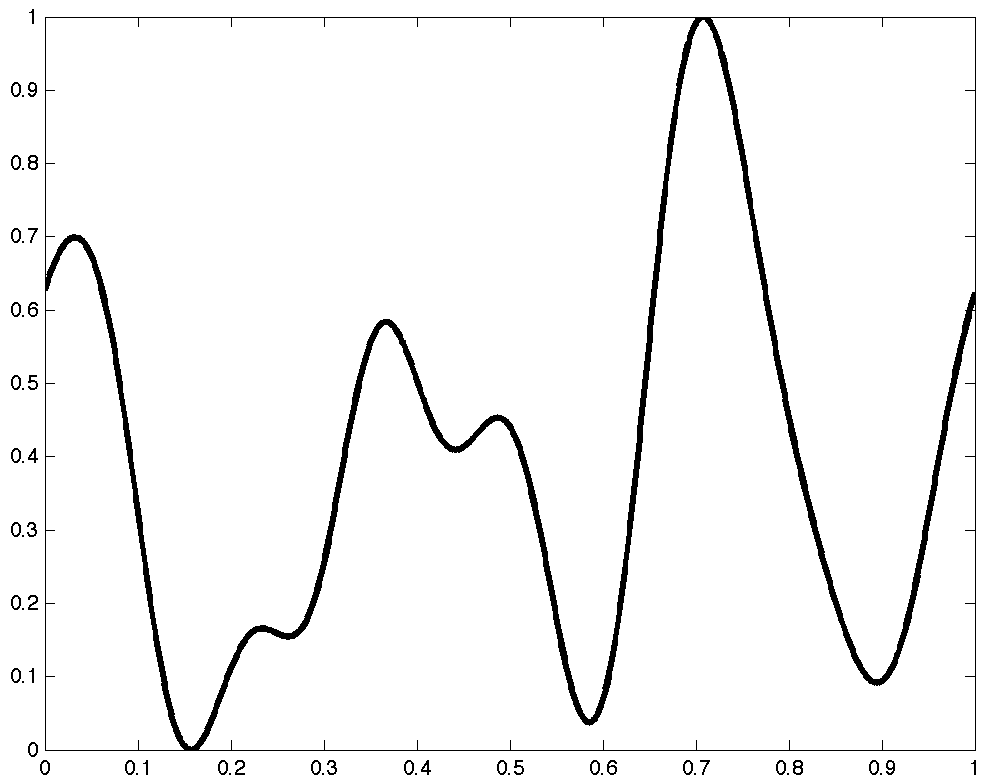
\includegraphics[width=0.4\linewidth]{manifold/regular1d/regular1d-function.png}&
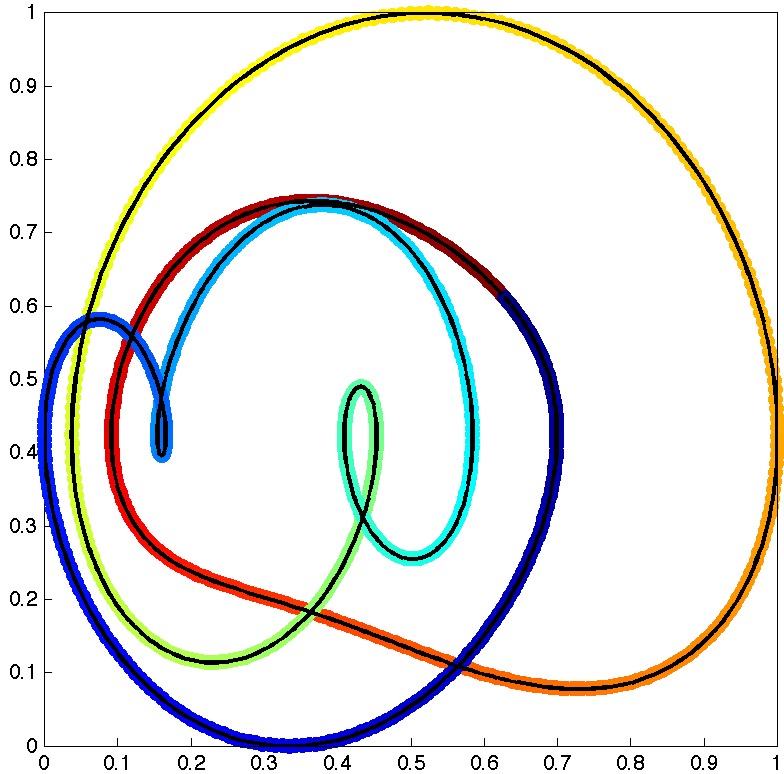
\includegraphics[width=0.32\linewidth]{manifold/regular1d/regular1d-manifold.png}\\
% \includegraphics[width=0.35\linewidth]{manifold/regular1d/regular1d-geodesic-dist.png}
%  & Distance $d_{\Mm}$\\[2mm]
Signal $f$ & Curve $\tilde c_f$
\end{tabular}
}{
Manifold of smooth signals.
%
}{fig-smooth-1d-manifold}


%%%%%%%%%%%%%%%%%%%%%%%%%%%%%%%%%%%%%%%%%%%%%%%%%%%%%%%%%%%%%%
\myparagraph{Uniformly regular 2D images.}
Smooth images $f$ with periodic boundary conditions are described using the 3D manifold $\Mm$ of affine images. The manifold $\Mm$ thus defines a surface 
\begin{equation*}
	\foralls x \in \zun^2, \quad \tilde \Cc_f(x_1,x_2) = \phi^{-1}( \Proj_\Mm(p_x(f)) ) \approx \pa{f(x), \pd{f}{x_1}, \pd{f}{x_2}} \in \RR^3.
\end{equation*}
Figure \ref{fig-smooth-image}, left, shows an example of a regular image, that is generated as a realization of a Gaussian random field $X$ whose power spectrum satisfies $|\hat X(\om)| = (1+|\om|)^{-r}$ for a regularity exponent $r>1$ (for the figure we have set $r=3$). 

Figure \ref{fig-smooth-image}, right, shows the corresponding 2D surface $\tilde c_f$ embedded in the 3D volume $\Om = \phi^{-1}(\Mm)$. This surface is topologically equivalent to a torus but exhibits self intersections along 1D curves. 

% On figure \ref{fig-smooth-image}, right, one can see the geodesic distance $x \mapsto d_{\Mm}(p_{x_0}(f),p_x(f))$ displayed as a 2D image since $x \in \zun^2$. This distance corresponds to the Euclidean distance over the cube $\phi^{-1}(\Mm)$, but since $\tilde c_f$ has a complex convoluted geometry, this distance is not Euclidean when displayed as a 2D image.

\myfigure{
\begin{tabular}{c@{\hspace{2mm}}c}

\includegraphics[width=0.28\linewidth]{manifold/regular2d/regular2d-original.png}&
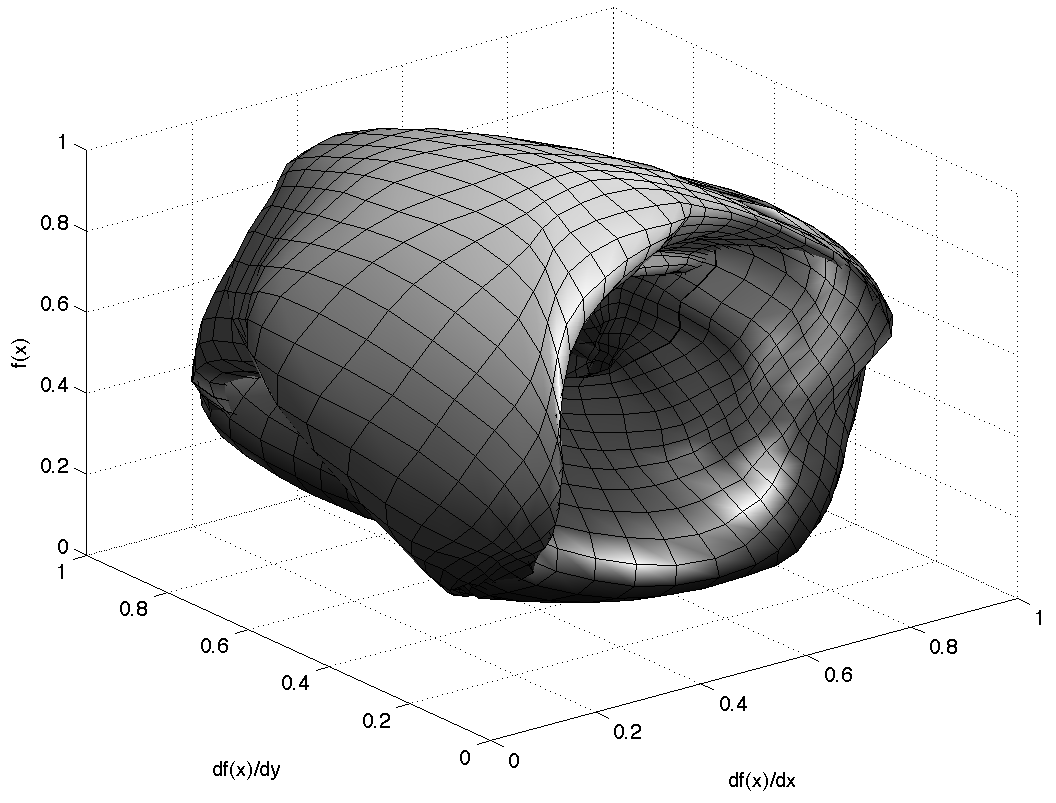
\includegraphics[width=0.4\linewidth]{manifold/regular2d/regular2d-manifold.png}\\
%\includegraphics[width=0.28\linewidth]{manifold/regular2d/regular2d-geodesic-dist.png}\\[-3mm]
Image $f$ & Surface $\tilde c_f$
\end{tabular}
}{
Manifold of smooth images.
%
}{fig-smooth-image}




%%%%%%%%%%%%%%%%%%%%%%%%%%%%%%%%%%%%%%%%%%%%%%%%%%%%%%%%%%%%%%
\subsection{Manifold of Cartoon Images}
\label{sec-manifold-cartoon-images}

Uniformly smooth signals and images are of little practical interest to model natural datasets. Signals with step discontinuities are efficiently processed with wavelets that avoid ringing artifacts of a linear Fourier approximation. 
Images with contours contain sharp variations along regular curves that make wavelets sub-optimal because of their square support \cite{mallat-book}.

A simple model of binary images is defined as
\begin{equation*}
	\Th = \enscond{ 1_{B} * h(x) }{ B \subset \zun^2 \text{ with } \partial B \text{ regular}}.
\end{equation*}
where $h$ is a regular kernel.
The set $B$ represents the object of interest in the scene. It is supposed to be connected with $\partial B$ of bounded curvature. This model can be extended to multiple objects as long as their boundaries are separated by a distance larger than $\tau$.

Locally a patch of $f$ is well approximated by a single straight edge 
\begin{equation*}
	p_x(f)(t) \approx P_{(\th(x),\de(x))}(t)
	\qqwhereqq
	P_{(\th,\de)}(t) = P\bpa{ R_{\th}(t - (\de,0)) },
\end{equation*}
where $R_{\th}$ is the planar rotation of angle $\th$. The step is $P = h * \tilde P$ where $\tilde P(t)=0$ if $t_1<0$ and $\tilde P(t)=1$ otherwise. Figure \ref{fig-edge-patches-samples} shows some examples of typical edge patches.

\myfigure{
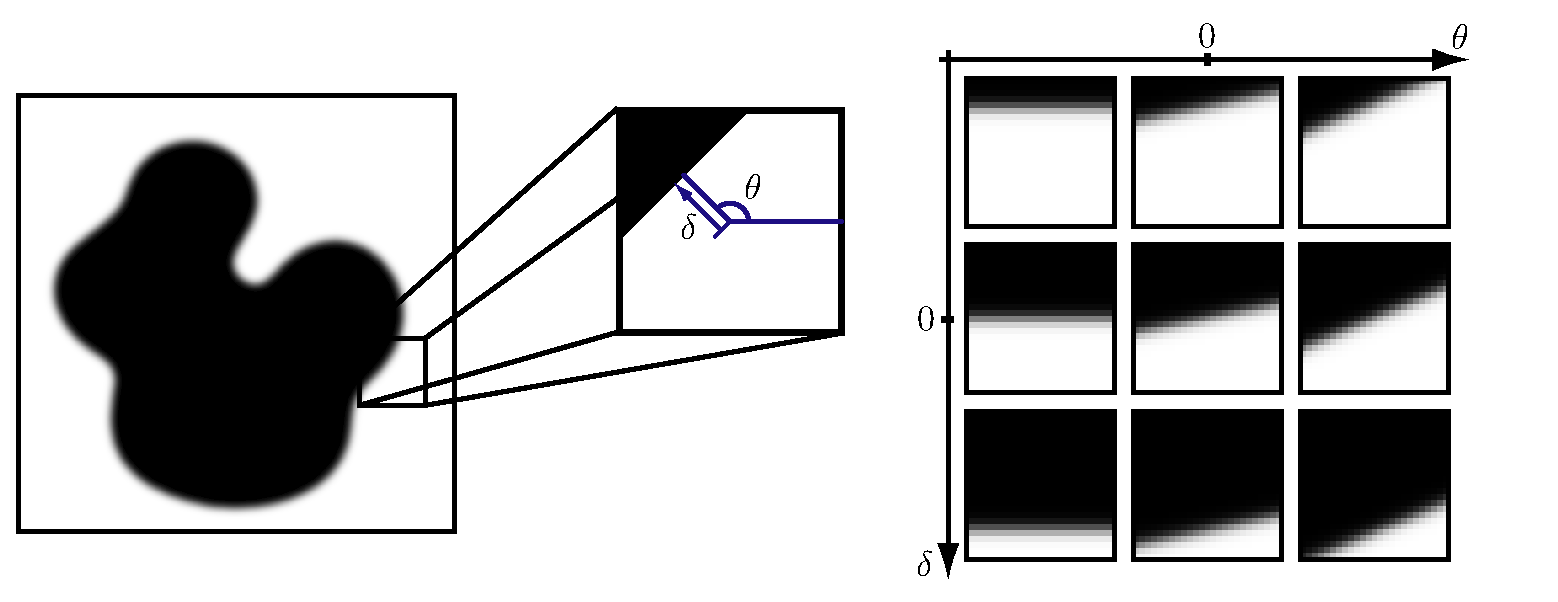
\includegraphics[width=0.8\linewidth]{manifold-edges/edge-manifold.eps}
}{
Left: an example of cartoon image. Right: parameterization of the manifold of edge patches and some examples.
%
}{fig-edge-patches-samples}


This leads to the following 2D parameterization of the manifold of binary edge patches
\eql{\label{eq-manifold-binary-edges}
	\phi : 
	\left\{
	\begin{array}{ccc}
		\Sun \times \RR^+ & \longrightarrow & \Mm\\
		(\th,\de) & \longmapsto & P_{(\th,\de)}.
	\end{array}
	\right.
}
The manifold $\Mm$ is thus topologically equivalent to a cylinder, however, due to the lack of translation invariance when the edge approaches the boundary of $[-\tau/2,\tau/2]^2$, the manifold is not flat. Indeed the two constant functions equal to 0 and 1 play a special role of poles. Figure \ref{fig-manifold-edges-2d} shows a 3D display of the corresponding embedding. We note that for this edge manifold, one generally has $\Mm = \tilde \Cc_f$ since the boundary $\partial B$ covers all the orientations $\th \in \Sun$. However the surface $\Cc_f$ traced by $f$ on the parameter domain $\Sun \times \RR^+$ is complex if $\partial B$ exhibits concavities that lead to self intersections of $\Cc_f$. Figure \ref{fig-manifold-edges-2d} shows curves that correspond to a 1D sections in $\Cc_f$. These curves trace closed loops on the manifold $\Mm$.

\myfigure{
\raisebox{.3cm}{ %
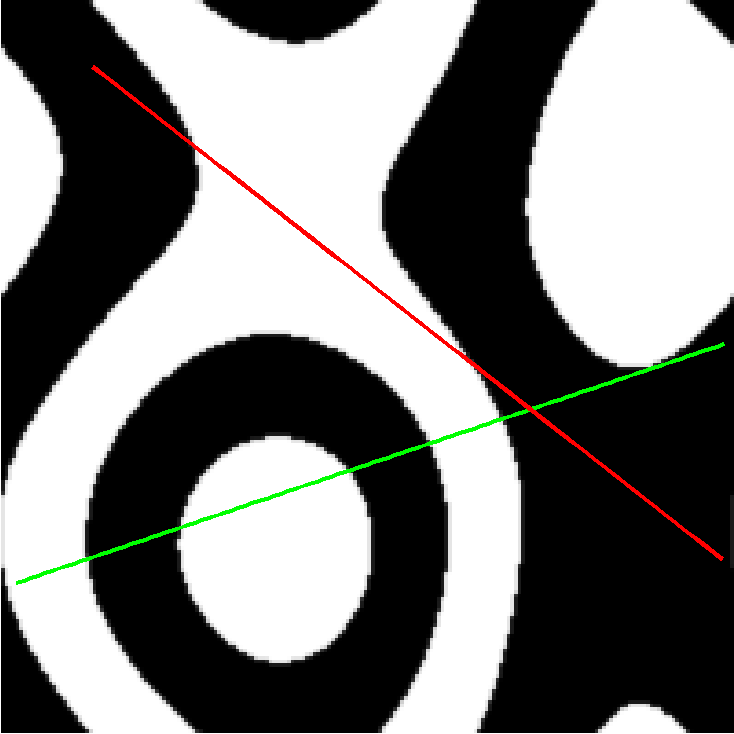
\includegraphics[width=0.35\linewidth]{manifold-edges/cartoon-curves.png} }\qquad\qquad
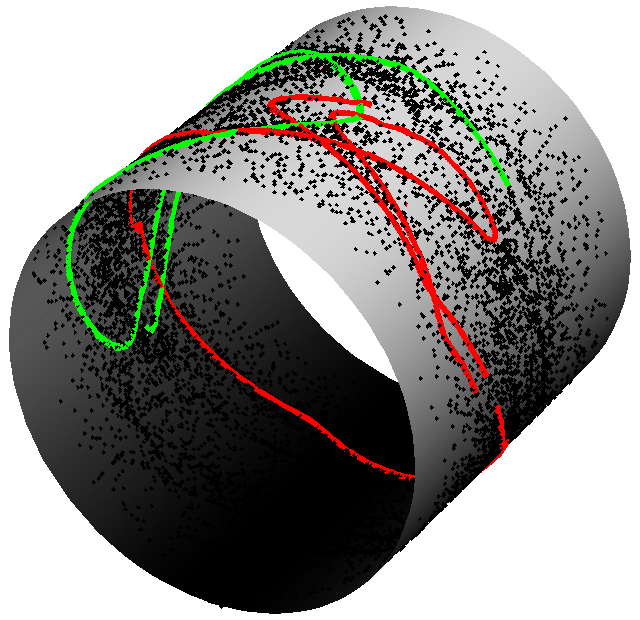
\includegraphics[width=0.4\linewidth]{manifold-edges/cartoon-manifold.png}
}{
Left: a cartoon image. Right: 3D representation of the edge manifold $\Mm$ (depicted in 3D as a cylinder). The two curves on the manifold corresponds to patches extracted along the two lines in the image.
%
}{fig-manifold-edges-2d}



%%%%%%%%%%%%%%%%%%%%%%%%%%%%%%%%%%%%%%%%%%%%%%%%%%%%%%%%%%%%%%
%%%%%%%%%%%%%%%%%%%%%%%%%%%%%%%%%%%%%%%%%%%%%%%%%%%%%%%%%%%%%%
%%%%%%%%%%%%%%%%%%%%%%%%%%%%%%%%%%%%%%%%%%%%%%%%%%%%%%%%%%%%%%
\subsection{Manifold of Locally Stationary Sounds}
\label{sec-manifold-oscillation-1d}

\newcommand{\Phase}{\Psi}

Natural sounds are usually modeled as highly oscillating signals with a phase that is slowly varying. Such a signal can be written as 
\begin{equation*}
	f(x) = A(x) \cos( \Phase(x) ),
\end{equation*}
where $A(x) \geq 0$ is the local amplitude, and $\Phase'(x) \geq 0$ the local phase of the oscillations. Such a decomposition is however non uniquely defined and one usually assumes that $A$ and $\Phase'(x)$ are slowly varying with respect to the signal sampling so that they can be reliably estimated. This leads to the following signals ensemble
\begin{equation*}
	\Th = 
	\enscond{ x \mapsto f(x) = A(x) \cos( \Phase(x) ) }{
		\norm{A'}_{\infty} \leq A_{\max} \qandq
		\norm{\Phase''}_{\infty} \leq \Phase_{\max}.
	}
\end{equation*}

Patches extracted from locally stationary signals are close to the manifold 
\begin{align*}
	\Mm & = \enscond{ P_{(A, \rho,\de)} }{ A \geq 0 \qandq \rho \geq 0 \qandq \de \in \Sun }\\
	\qwhereq
	& P_{(A,\rho,\de)}(x) = A \cos( \rho x + \de ).
\end{align*}
The parameterization $(A, \rho,\de) \mapsto P_{(A, \rho,\de)}$ shows that $\Mm$ is equivalent to $\Om = \RR^+ \times \RR^+ \times \Sun$.

The projection of a patch $p \in \Ldeux([-\tau/2,\tau/2])$ on $\Mm$ can be carried over approximately using a windowed Fourier transform. One uses a smooth window function $h$ supported on $[-\tau/2,\tau/2]$ and defines the windowed Fourier transform of $p$
\eq{
	\hat p(\om) = \int h(t) p(t) \exp(-\imath \om t) \d t.
}
Following Delprat et al. \cite{delprat-asymptotic} (see also \cite{mallat-book}), the projection of $p$ is then given as
\eql{\label{eq-spectrogram-estimation}
	\Proj_{\Mm}(p) \approx P_{(A,\rho,\de)}
	\qwhereq
	\choice{
		\rho = \underset{\om \geq 0}{\text{argmax}} \; |\hat p(\om)| \\
		\hat p(\rho) = A \exp(\imath \de).
	}
}
A 1D signal $f$ defines a 1D curve $\tilde c_f \subset \Mm$ traced on the manifold and a 1D curve $\tilde \Cc_f$ in 3D parameter space
\eq{
	\tilde \Cc_f = \{�(A(x), \rho(x),\de(x)) \}_{x \in [0,1]}
	\qwhereq
	P_{(A(x), \rho(x),\de(x))} = \Proj_{\Mm}( p_x(f) ).
}	
Figure \ref{fig-oscillations-1d} shows examples of a locally stationary oscillating signal together with its spectrogram and the corresponding curve $\tilde \Cc_f$ over the parametric space.

\myfigure{
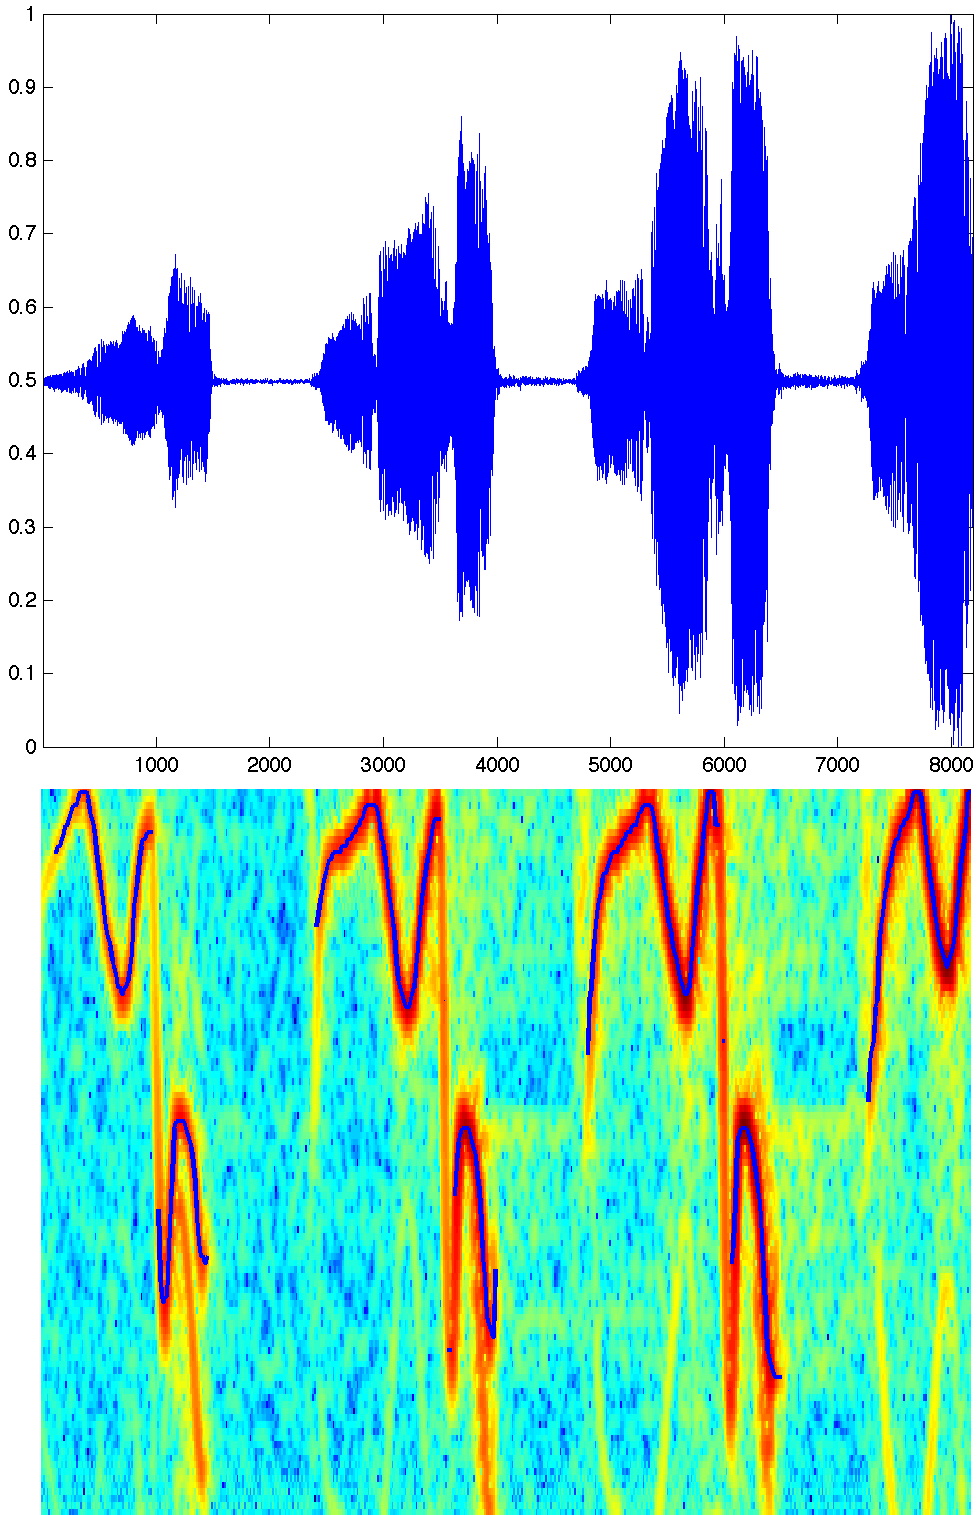
\includegraphics[width=0.37\linewidth]{manifold/bird/bird-sound-spectrogram.png}\hspace{2mm}
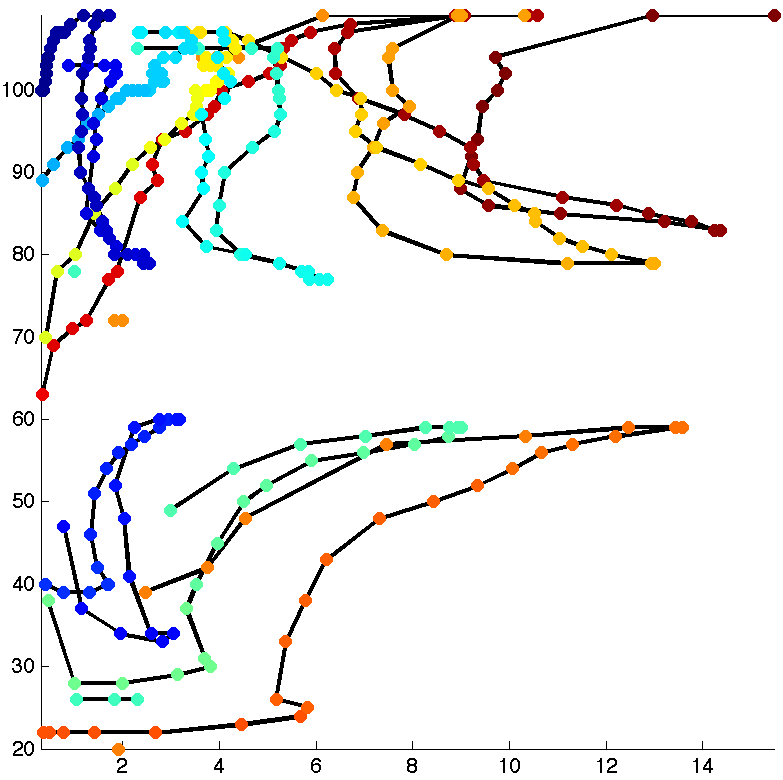
\includegraphics[width=0.57\linewidth]{manifold/bird/bird-manifold.png}
\vspace{2mm}
}{
Upper-left: 1D signal of a bird singing, bottom left: the corresponding log-spectrogram $\log(|\hat p_x(f)(\om)|)$ (the blue curve is the maxima curve $(x,\rho(x))$), right: the 2D curve $(A(x),\rho(x))$. For the display, the curve has been disconnected in areas where the bird stop singing (characterized by a low value of $A(x)$).
}{fig-oscillations-1d}





%%%%%%%%%%%%%%%%%%%%%%%%%%%%%%%%%%%%%%%%%%%%%%%%%%%%%%%%%%%%%%
%%%%%%%%%%%%%%%%%%%%%%%%%%%%%%%%%%%%%%%%%%%%%%%%%%%%%%%%%%%%%%
%%%%%%%%%%%%%%%%%%%%%%%%%%%%%%%%%%%%%%%%%%%%%%%%%%%%%%%%%%%%%%
\subsection{Manifold of Locally Parallel Textures}
\label{sec-manifold-locpar-textures}

Some natural textures are composed of nearly parallel stripes that are modeled as local oscillations. A locally parallel texture is defined as $f(x) = A(x) h( \Phase(x) ) + B(x)$ where $\nabla_x \Phase$ controls the direction and frequency of the oscillations around the point $x$, $A(x)$ is a local amplitude, $B(x)$ a local shift, and $h : \RR \rightarrow \RR$ is the periodic 1D profile of the oscillations.  This model of locally parallel textures is the extension of locally stationary sounds to images, if one considers the case $h(x) = \cos(x)$. Figure \ref{fig-manifold-examples}, right, shows examples of locally parallel textures. 

A local texture patch is approximated as
\begin{equation*}
	p_x(f) \approx P_{(A(x),B(x),\rho(x),\th(x),\de(x))}^h
	\qwhereq
	P_{(A,B,\rho,\th,\de)}^h(x) = A h( \rho \dotp{x}{\th} + \de ) + B.
\end{equation*}
The parameter $\th \in \tSun$ is the direction of the oscillations, $\rho$ their frequency and $\de$ is a phase shift. The manifold $\Mm$ is parameterized as
\eql{\label{eq-defn-oscillations-2d}
	\phi : 
	\left\{
	\begin{array}{ccc}
		\RR^+ \times \RR \times \RR^+ \times \tSun \times \Sun & \longrightarrow & \Mm\\
		(A,B,\rho,\th,\de) & \longmapsto & P_{(A,B,\rho,\th,\de)}^h.
	\end{array}
	\right.
}
An approximate estimation of $(\rho(x),\th(x),\de(x))$ from a texture $f$ can be carried over using local Fourier expansions over windows of size $\tau$ as defined in the 1D case in equation \eqref{eq-spectrogram-estimation}. 

\myfigure{
\begin{tabular}{c@{\hspace{2mm}}c@{\hspace{2mm}}c}
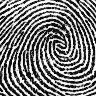
\includegraphics[width=.32\linewidth]{locpar-approx/fingerprint3-original.png}&
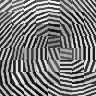
\includegraphics[width=.32\linewidth]{locpar-approx/fingerprint3-w12.png}&
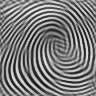
\includegraphics[width=.32\linewidth]{locpar-approx/fingerprint3-w2.png}\\
Image $f$ & Subsampling & $\Proj_{\Mm}(f)$
\end{tabular}
}{
An image and its projection $\Proj_{\Mm}(f)$ on the manifold model of oscillating textures. The center image displays a projection computed with a subset of non-overlapping patches $p_x(f)$, to better see the importance of translation invariance.
}{fid-locpar-approx}

The feature manifold depends on the specific choice of the profile $h$
\eq{
	\Mm = \Mm_h = \enscond{ P_{(A,B,\rho,\th,\de)}^h }{ (A,B,\rho,\th,\de) \in \Om  }.
}
An adaptation of the manifold to an exemplar $f \in \Ldeux([0,1]^d)$ to process is achieved by optimizing the profile $h$ so that the patches of $\fe$ are as close as possible from the manifold $\Mm_h$. This amount to minimizing the energy $E_{\Mm_h}$ defined in \eqref{eq-defn-energy-manifold} to select an adapted profile $h^\star$
\eql{\label{eq-adaptation-texture}
	h^\star = \uargmin{h \in H} E_{\Mm_h}(\fe),
}
where $H \subset \Ldeux(\RR)$ is a set of profiles, that might for instance contains some smoothness constraints on the texture profile.

We restrict the computation to a simple set of 1D profiles parameterized by a contrast $\gamma \in (0,1]$
\eql{\label{eq-profile-texture}
	h_\ga(x) = \sign(\cos(x)) | \cos(x)|^\gamma.
}
The optimal $\gamma$ minimizing $E_{\Mm_{h_\ga}}(f)$ is computed by testing a discrete set of values in $(0,1]$. Figure \ref{fid-locpar-approx} shows examples of projection with $\ga=0.35$, which is the value minimizing $E_{\Mm_{h_\ga}}(f)$ for the fingerprint image $f$. More elaborated adaptation strategies could be used to fit arbitrary texture profiles.





%%%%%%%%%%%%%%%%%%%%%%%%%%%%%%%%%%%%%%%%%%%%%%%%%%%%%%%%%%%%%%
%%%%%%%%%%%%%%%%%%%%%%%%%%%%%%%%%%%%%%%%%%%%%%%%%%%%%%%%%%%%%%
%%%%%%%%%%%%%%%%%%%%%%%%%%%%%%%%%%%%%%%%%%%%%%%%%%%%%%%%%%%%%%
\subsection{Manifold of Sparse Patches}
\label{subsec-sparse-patches}


%%%%%%%%%%%%%%%%%%%%%%%%%%%%%%%%%%%%%%%%%%%%%%%%%%%%%%%%%%%%%%
\myparagraph{Sparse patch expansion.}
The sparse patch model assumes that each patch $p_x(f)$ extracted from a signal or image $f$ has a sparse expansion 
\eq{
	p_x(f) = \sum_i s_x(i) \phi_i = D s_x
}
using a dictionary $D = \{ \phi_i \}_{i=0}^{P-1}$ of $P$ atoms. Each $\phi_i \in \Ldeux([-\tau/2,\tau/2]^d)$ is an atomic template and $s_x(i) \in \RR$ is the corresponding coefficient. The sparsity of the decomposition is ensured by constraining the $\lzero$ pseudo-norm of the coefficients to be smaller than $S \in \NN^*$
\begin{equation*}
	\norm{s_x}_{\lzero} = \#\enscond{i}{s_x(i) \neq 0} \leq S.
\end{equation*}
This leads to the manifold of sparse patches
\eq{
	\Mm = \Mm_D = \enscond{ \sum_i s(i) \phi_i }{ \norm{s}_{\lzero} \leq S }.
}
This set $\Mm$ is not a smooth manifold but rather a non-linear union of $S$-dimensional linear spaces. It is parameterized by the dictionary $D$ and the sparsity level $S$. 

The corresponding signal ensemble $\Th$ with sparse patches is 
\eql{
	\label{eq-sparsity-texture}
	\Theta = \Theta_D = \enscond{f}{\foralls x, \; p_x(f) = D s_x \qwithq \norm{s_x}_{\lzero} \leq S}
}
This model has been introduced by Peyr\'e \cite{peyre-sparse-textures} for texture synthesis and is re-casted in our manifold patch model.

The projection on the sparse manifold $\Mm$ requires the computation of 
\begin{equation*}
	\Proj_{\Mm}(p) = D \, \uargmin{s \in \RR^{m}} \norm{p-D s}_{\ldeux}
			\quad \text{subject to} \quad
			\norm{s}_{\lzero} \leq S.
\end{equation*}
The exact computation of this projection is NP-hard for an arbitrary dictionary $D$, but it can be solved approximately using for instance $S$ steps of orthogonal matching pursuit algorithm, see \cite{mallat-book}.


%%%%%%%%%%%%%%%%%%%%%%%%%%%%%%%%%%%%%%%%%%%%%%%%%%%%%%%%%%%%%%
\myparagraph{Dictionary learning.}
The manifold $\Mm_D$ is optimized so that a given exemplar $\fe$ is as close as possible to $\Th_D$. This corresponds to the learning of the dictionary $D$, that is optimized in order to minimize the goodness of fit of $\fe$ to the model generated by $D$
\eql{\label{eq-optimal-dictionary}
	D^\star = \uargmin{D} E_{\Mm_D}(\fe)
}
where the energy $E_{\Mm_D}$ is defined in \eqref{eq-defn-energy-manifold}. This is similar to the adaptation of the profile to optimize the oscillating texture model \eqref{eq-adaptation-texture}. In the optimization \eqref{eq-optimal-dictionary}, the atoms $\phi_i$ of $D$ are only constrained to be of unit norm, $\norm{\phi_i} = 1$.

The optimization \eqref{eq-optimal-dictionary} is re-written by optimizing over both the dictionary $D$ and the coefficients $s_x$ of the patches $p_x(\fe)$
\eql{
	(D^\star, \{s_x^\star\}_x) = \uargmin{D, \{s_x\}_x} \sum_x \norm{ p_x(\fe) - D s_x }^2
	\qsubjq
	\norm{s_x}_{\lzero} \leq S.
}
This optimization problem is highly non-convex and a stationary point of $E_{\Mm_D}$ with respect to $D$ can be computed using several iterative algorithms, for instance the MOD algorithm \cite{engan-mod} or K-SVD \cite{aharon-ksvd}. Table \ref{listing-dictionary-learning} details the MOD optimization process, that alternates between the computation of the coefficients $\{s_x\}_x$ and the optimization of the dictionary atoms $\phi_i$. 

\begin{listing}
\begin{enumerate}
	\item \textit{Initialization:} set each $\phi_i$ as a realization of a white noise, normalized so that $\norm{\phi_i}=1$.
	\item \textit{Coefficient update:} compute the projection $D s_x$ of each patch $p_x(\fe)$, on the manifold $\Mm$ 
		\begin{equation*}
			s_x = \uargmin{s} \norm{ p_x(\fe) - D s} \qsubjq \norm{s}_{\lzero} \leq S.
		\end{equation*}
		This is computed approximately with $S$ steps of orthogonal matching pursuit applied to $p_x(\fe)$.
	\item \textit{Dictionary update:} the dictionary $D$ is computed by minimizing
		\eq{
			\umin{D} \sum_x \norm{ p_x(\fe) - D s_x }^2,
		}
		whose solution is given as
		\eq{
			D \leftarrow \Pi \Si^{+} \qqwhereqq
			\Si+ = (\transp{\Si} \Si)^{-1} \transp{\Si}
		}
		where $\Si = \{s_x\}_x$ is the matrix whose columns are the coefficients $s_x$ and 
		$\Pi = \{ p_x(\fe) \}_x$ is the matrix whose columns are the (discretized) patches $p_x(\fe)$.
	\item \textit{Normalization:} for all $i$, $\phi_i \leftarrow \phi_i/\norm{\phi_i}$. 
	\item \textit{Stop:} while not converged, go back to 2. 
\end{enumerate}% \vspace{-3mm}
    \caption{MOD dictionary learning algorithm. \label{listing-dictionary-learning}}
\end{listing}

Figure \ref{fig-dictionary-learning} shows an example of a dictionary learned from an homogeneous texture.

\myfigure{
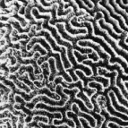
\includegraphics[width=0.3\linewidth]{dictionary-learning/corral-original.png} 
\itemraise{2cm}{ %
	$\overset{\text{learning}}{\longrightarrow}$ }
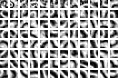
\includegraphics[width=0.46\linewidth]{dictionary-learning/corral-dictionary-r02s02.png}
\vspace{2mm}
}{
Left: input texture $\fe$, 
right: dictionary $D$ learned to sparsity the patches $p_x(\fe)$.
%
}{fig-dictionary-learning}




%%%%%%%%%%%%%%%%%%%%%%%%%%%%%%%%%%%%%%%%%%%%%%%%%%%%%%%%%%%%%%
%%%%%%%%%%%%%%%%%%%%%%%%%%%%%%%%%%%%%%%%%%%%%%%%%%%%%%%%%%%%%%
%%%%%%%%%%%%%%%%%%%%%%%%%%%%%%%%%%%%%%%%%%%%%%%%%%%%%%%%%%%%%%
\section{Inverse Problem Regularization with Manifold Models}
\label{sec-inverse-pbm}


%%%%%%%%%%%%%%%%%%%%%%%%%%%%%%%%%%%%%%%%%%%%%%%%%%%%%%%%%%%%%%
\subsection{Inverse Problems}

The manifold prior model introduced in Section \ref{subsec-global-manif-model} is used to regularize the inversion of an operator $\Phi : \Ldeux(\zd) \rightarrow V$, where $V$ is an Hilbert space of finite or infinite dimension. The mapping $\Phi$ is typically ill-posed and difficult to invert since $\Phi f$ gathers only a limited amount of information from the original $f$ to recover. 

Forward measurements correspond to the computations of
\begin{equation*}
	y = \Phi f + \epsilon \in V,
\end{equation*}
where $f$ is the data to recover and $\epsilon$ is an additive noise.

Regularization theory assumes that $f$ belongs to some functional space $H$ such as a Sobolev space (linear regularization) or the space of bounded variations (non-linear regularization). The recovered signal $f^\star$ is the solution of an optimization problem
\eql{\label{eq-regularized-inversion}
	f^\star = \uargmin{g \in H} \norm{y-\Phi g}^2 + \la E(g),
}
where $E$ should be small when $g$ is close to the smoothness model. The weight $\la$ should be adapted to match the amplitude of the noise $\epsilon$, which might be a non-trivial task in practical situations. 

Classical variational priors include
\begin{rs}
	\item \textit{Total variation:} The bounded variation model imposes that $f^\star$ has a finite bounded variation and uses 
	\eql{\label{eq-defn-tv-prior}
		E(g) = \normTV{g} = \int |\nabla_x g| \d x.
	}
	This prior has been introduced by Rudin, Osher and Fatemi \cite{rudin-tv} for denoising purpose. 
	\item \textit{Sparsity priors:} Given an orthogonal basis $\{\psi_k\}_{k}$ of $\Ldeux(\zd)$, a sparsity enforcing prior is defined as
	\eql{\label{eq-defn-sparsity-prior}
		E(g) = \sum_k |\dotp{g}{\psi_k}|.
	}
	This prior has been introduced by Donoho and Johnstone \cite{donoho-shrinkage} with the wavelet basis for denoising purpose. It has then been used to solve more general inverse problems, see for instance \cite{daubechies-iterated} and the references therein. It can also be used in conjunction with redundant frames instead of orthogonal bases, see for instance~\cite{starck-inpainting,fadili-inpainting-cj}.
\end{rs}


%%%%%%%%%%%%%%%%%%%%%%%%%%%%%%%%%%%%%%%%%%%%%%%%%%%%%%%%%%%%%%
\subsection{Regularization with Manifold Model}
\label{subsec-regularize-manifold}

This paper explores the global manifold energy $E = E_{\Mm}$ defined in equation \eqref{eq-defn-energy-manifold} to perform the regularization.
The optimization \eqref{eq-regularized-inversion} with $E=E_{\Mm}$ is performed by introducing a manifold valued function $c^\star \in \Vv(\Mm)$. At each location $x$, the patch $c^\star(x) \in \Mm$ is tracking a local feature of $f^\star$ and should be close to $p_x(f)$. 

The optimization \eqref{eq-regularized-inversion} is re-written using $c^\star$ as
\begin{align}
	\label{eq-optimization-extended}
	& (f^\star,c^\star) = \uargmin{(g,c) \in \Ldeux(\zd) \times \Vv(\Mm)} \Ee_{\Mm}(g,c),\\
	 \qwhereq
	&\Ee_{\Mm}(g,c) = \norm{y-\Phi g}^2 + \la \int_{\zd} \norm{p_x(g) - c(x)}^2 \d x
\end{align}
whose solution $f^\star$ also solves the original problem \eqref{eq-regularized-inversion} for $E = E_{\Mm}$, and $c^\star = \tilde c_{f^\star}$.

The manifold valued mapping $c^\star$ should be close to the original projected curve (or surface when $d=2$) $\tilde c_f$ as defined in \eqref{eq-curve-manifold-projected}. The manifold regularization of inverse problems \eqref{eq-optimization-extended} computes a curve (or surface) traced on the manifold $\Mm$ that also matches the forward measurements $y$.

A stationary point of \eqref{eq-optimization-extended} is computed by alternatively minimizing over $f^\star$ and $c^\star$:
\begin{rs}
	\item \textit{The image is fixed.} The manifold valued function $c_0$ minimizing 
		$\Ee_{\Mm}(g,c)$ with respect to $c \in \Vv(\Mm)$ is computed with 
		 the projection defined in equation \eqref{eq-defn-manifold-proj}
		\eql{\label{eq-defn-manifold-proj-iteration}
			\foralls x \in \zd, \quad c_0(x) = \Proj_{\Mm}(p_x(g)).
		}
	\item \textit{The manifold-valued mapping is fixed.} 
		The signal $g_0$ minimizing
		$\Ee_{\Mm}(g,c)$ with respect to $g \in \Ldeux(\zd)$ is the solution of 
		\eq{
			(\transp{\Phi}\Phi + \la \Id) g_0 = \transp{\Phi} y + \la \text{Aver}(c)
		}
		where the averaged signal $\text{Aver}(c) \in \Ldeux(\zd)$ of $c$ is defined in \eqref{eq-averaging}.
\end{rs}
The iteration of these two steps corresponds to the manifold pursuit detailed in table \ref{listing-iterative-projection}. 

\begin{listing}
\begin{enumerate}
	\item \textit{Initialization:} set $f^{(0)} = \transp{\Phi} y$ and $k \leftarrow 0$.
	\item \textit{Manifold closest point:} update the manifold valued function as
		\eq{
			\foralls x \in \zd, \quad c^{(k+1)}(x) = \Proj_{\Mm}( p_x(f^{(k)}) ),
		}
		where the manifold projection $\Proj_{\Mm}$ is defined in \eqref{eq-defn-manifold-proj}.
	\item \textit{Least square fit:} update the current estimate as
		\eq{
			f^{(k+1)} = (\transp{\Phi}\Phi + \la \Id)^{-1} \pa{ \transp{\Phi} y + \la \text{Aver}(c^{(k+1)}) }.
		}
		and where the averaging $\text{Aver}(c^{(k+1)})$ of $c^{(k+1)}$ is defined in \eqref{eq-averaging}.
	\item \textit{Stopping criterion:} while not converged, set $k \leftarrow k+1$ and go back to 2.
\end{enumerate}% \vspace{-3mm}
    \caption{Manifold pursuit to minimize \eqref{eq-optimization-extended}. \label{listing-iterative-projection}}
\end{listing}

The algorithm of table \ref{listing-iterative-projection} shares some similarities with iterative thresholdings methods used to solve the non-linear regularized inversion \eqref{eq-regularized-inversion} with a sparsity prior \eqref{eq-defn-sparsity-prior}, see for instance~\cite{daubechies-iterated}. To handle the noiseless case $\epsilon=0$, the value of the regularization parameter $\la$ can be decreased toward $0$ during the iterations.

The main computational burden in the manifold pursuit is the numerical computation of the projection $\Proj_{\Mm}$ on the manifold. Depending on the image model considered, specific solvers can be used. For complex manifolds without any analytical description, a dense sampling of the manifold is used together with a fast closest-point algorithm.

Since the energy to optimize \eqref{eq-optimization-extended} is non-convex, the manifold pursuit might fail to converge to the global minimizer of the problem. For a smooth manifold $\Mm$, the iterates $(f^{(k)},c^{(k)})$ of the algorithm \ref{listing-iterative-projection} converge to a stationary point $(f^\star,c^\star)$ of the energy $\Ee_{\Mm}$ since this energy satisfies the hypotheses of \cite{tseng-proximal}. 

% This paper shows various numerical simulations for several manifold models in order to validate the usefulness of the approach and the efficiency of the algorithm. 


%%%%%%%%%%%%%%%%%%%%%%%%%%%%%%%%%%%%%%%%%%%%%%%%%%%%%%%%%%%%%%
%%%%%%%%%%%%%%%%%%%%%%%%%%%%%%%%%%%%%%%%%%%%%%%%%%%%%%%%%%%%%%
%%%%%%%%%%%%%%%%%%%%%%%%%%%%%%%%%%%%%%%%%%%%%%%%%%%%%%%%%%%%%%
\subsection{Numerical Experiments}

Although any linear operator can be treated within our regularization framework, this paper focusses on the following examples.
\begin{rs}
	\item \textit{Inpainting} corresponds to the operation of removing pixels from an input data
	\eq{
		(\Phi f)(x) = 
		\choice{
			0 \qifq x \in \Omega,\\
			f(x) \qifq x \notin \Omega,
		}
	}
	where $\Om \subset \zd$ is the region where the input data has been damaged. Classical methods for inpainting use partial differential equations that propagate the information from the boundary of $\Om$ to its interior, see for instance \cite{masnou-level-lines,ballester-filling,bertalmio-inpainting,tschumperle-inpainting}. Sparsity promoting prior such as \eqref{eq-defn-sparsity-prior} in wavelets frames and local cosine bases have been used to solve inpainting as a inverse problem \cite{starck-inpainting,fadili-inpainting-cj}.
	
	\item \textit{Compressive sensing} is a new sampling theory that uses a fixed set of linear measurements together with a non-linear reconstruction \cite{candes-near-optimal,donoho-cs}, see also the review \cite{candes-cs-review}.	
	The sensing operator computes the projection of the data on a finite set of $k$ vectors
		\eql{\label{eq-defn-cs}
			\Phi f = \{ \dotp{f}{u_i} \}_{i=0}^{k-1} \in \RR^k.
		}
		The signal are discretized finite dimensional vectors $f \in \RR^n$.
		Compressive sensing states hypotheses on both the input signal $f$ and the sensing vectors $\{ u_i \}_i$ for this non-uniform sampling process to be invertible with $\lun$ minimization. The sensing vectors $\{ u_i \}_i$ must be incoherent, which is the case with high probability if they are drawn randomly from unit norms Gaussian white noise vectors. Under the additional condition that $f$ is sparse in some orthogonal basis $\{\psi_k\}_k$
		\eq{\label{cs-recovery}
			\#\enscond{k}{\dotp{f}{\psi_k}\neq 0} \leq S, 
		}
		the optimization of \eqref{eq-regularized-inversion} with the sparsity prior \eqref{eq-defn-sparsity-prior} leads to a perfect recovery $f^\star=f$ if $k = O( S \log(n/S) )$, where $n$ is the dimension of the sampled signal $f$. This result holds in the noiseless case $\epsilon=0, \la \rightarrow 0$ and can be extended to an approximate recovery in the noisy case $\epsilon \neq 0, \la > 0$. 
\end{rs}

The following numerical experiments compare the efficiency of sparsity regularization with $\lun$ prior \eqref{eq-defn-sparsity-prior} with the patch manifold energy $E_\Mm$ \eqref{eq-defn-energy-manifold}. Sparsity regularization leads to a convex optimization, which is an advantage over the non-convex manifold regularization that might be trapped in a local minimum.

For numerical computation, discretized signals and images are obtained by an uniform sampling at $n$ points. The corresponding manifolds of patches $\Mm \subset \RR^{\tau^d n}$ are embedded in a finite dimensional space. The following numerical experiments are performed with patches of width $w=10$ pixels. Compressive sensing experiments are performed with sensing vectors $u_i$ that are random discrete Fourier vectors, so that the sensing operator $\Phi$ is computed with the FFT algorithm.

%%%%%%%%%%%%%%%%%%%%%%%%%%%%%%%%%%%%%%%%%%%%%%%%%%%%%%%%%%%%%%
\myparagraph{Smooth images.}
Figure \ref{fig-inpainting-fnoise} shows iterations of the algorithm \ref{listing-iterative-projection} to solve the inpainting problem on a smooth image using a manifold prior with 2D linear patches, as defined in \ref{eq-defn-manifold-smooth-variations}, with a low amplitude noise $\epsilon$. This manifold regularization together with the overlapping of the patches performs a smooth interpolation of the missing pixels. 

The iterations of the algorithm are similar to a linear diffusion that propagates the available information inside the set $\Om$ of removed pixels. The performances of the algorithm are similar to linear methods such as inpainting with a Sobolev regularizer $E(f) = \int |\nabla f|^2$ that corresponds to a heat diffusion inside $\Om$.


\myfigure{
\begin{tabular}{c@{\hspace{2mm}}c@{\hspace{2mm}}c@{\hspace{2mm}}c}
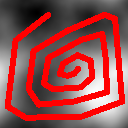
\includegraphics[width=0.24\linewidth]{inpainting/fnoise/fnoise-mask.png} &
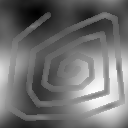
\includegraphics[width=0.24\linewidth]{inpainting/fnoise/fnoise-iter-001.png} &
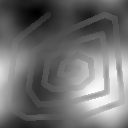
\includegraphics[width=0.24\linewidth]{inpainting/fnoise/fnoise-iter-002.png} &
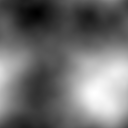
\includegraphics[width=0.24\linewidth]{inpainting/fnoise/fnoise-iter-150.png}\\
Measurements $y$ & Iter. \#1 & Iter. \#3 & Iter. \#50
\end{tabular}
}{
Iterations of the inpainting algorithm on an uniformly regular image.
%
}{fig-inpainting-fnoise}

%%%%%%%%%%%%%%%%%%%%%%%%%%%%%%%%%%%%%%%%%%%%%%%%%%%%%%%%%%%%%%
\myparagraph{Cartoon images.}
Figures \ref{fig-inpainting-disk} and \ref{fig-cs-disk} show iterations of the projection algorithm \ref{listing-iterative-projection} with a manifold model of binary edges, as defined in equation \eqref{eq-manifold-binary-edges}. For this numerical optimization, the manifold of edges is discretized as already done for the display of figure \ref{fig-manifold-edges-2d} and the projection $\Proj_{\Mm}$ is computed with a fast nearest-neighbor search. For both inpainting and compressive sampling, the manifold of edges allows to reconstruct with good precision the boundary of a single smooth object (here a disk).

\myfigure{
\begin{tabular}{c@{\hspace{2mm}}c@{\hspace{2mm}}c@{\hspace{2mm}}c}

\includegraphics[width=0.24\linewidth]{inpainting/disk/disk-mask.png} &
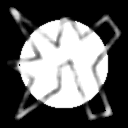
\includegraphics[width=0.24\linewidth]{inpainting/disk/disk-iter-001.png} &

\includegraphics[width=0.24\linewidth]{inpainting/disk/disk-iter-002.png} &

\includegraphics[width=0.24\linewidth]{inpainting/disk/disk-iter-013.png}\\
Measurements $y$ & Iter. \#1 & Iter. \#3 & Iter. \#50
\end{tabular}
}{
Iterations of the inpainting algorithm on a geometrical image with the binary edge model.
%
}{fig-inpainting-disk}


\myfigure{
\begin{tabular}{c@{\hspace{2mm}}c@{\hspace{2mm}}c@{\hspace{2mm}}c}
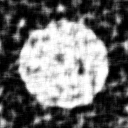
\includegraphics[width=0.24\linewidth]{compressive-sampling/disk/disk-iter-001.png} &

\includegraphics[width=0.24\linewidth]{compressive-sampling/disk/disk-iter-002.png} &
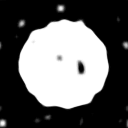
\includegraphics[width=0.24\linewidth]{compressive-sampling/disk/disk-iter-003.png} &

\includegraphics[width=0.24\linewidth]{compressive-sampling/disk/disk-iter-019.png}\\
Iter. \#1 & Iter. \#2 & Iter. \#3 & Iter. \#50
\end{tabular}
}{
Iterations of the compressive sensing reconstruction algorithm on a geometrical image with the binary edge model.
The number of sensed vectors is $n_0 = n/10$ where $n$ is the number of pixels. %
}{fig-cs-disk}

Figure \ref{fig-geometrical-cs} shows a more challenging compressive sensing problem where the image is composed of layers of occluding objects with smooth boundaries and varying intensities. In order to cope with a non-binary image, the manifold of affine edges is used
\eql{\label{eq-defn-affine-edges}
	\Mm  = \enscond{a P_{(\th,\de)} + b}{(\th,\de) \in \Sun \times \RR^+ \qandq (a,b) \in \RR^+ \times \RR}.
}
This manifold is four dimensional, but the projection on this manifold is computed efficiently by iteratively optimizing the projection over the $(\th,\de)$ parameters and then the $(a,b)$ parameters. Patches extracted from figure \ref{fig-geometrical-cs}, left, are however not always close to this manifold because of crossings that occur when two singularity curves meet. 

Figure \ref{fig-geometrical-cs} compares the compressive sensing reconstruction with a sparsity prior \eqref{eq-defn-sparsity-prior} in a translation invariant wavelet frame (center) and with a manifold prior in the affine edges manifold \eqref{eq-defn-affine-edges}. The optimization of the sparsity energy \eqref{eq-defn-sparsity-prior} is performed with an iterative thresholding algorithm, see \cite{daubechies-iterated}, whereas the optimization of the manifold energy \eqref{eq-optimization-extended} is performed with the algorithm \ref{listing-iterative-projection}. The reconstruction with a manifold prior is of better quality than the sparsity prior in a wavelet frame. This is because, in 2D, wavelets cannot take advantage of the regularity of the boundaries of the objects. 


\myfigure{
\begin{tabular}{c@{\hspace{2mm}}c@{\hspace{2mm}}c}
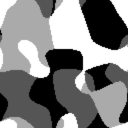
\includegraphics[width=0.32\linewidth]{compressive-sampling/geometrical/geometrical-original.png} &
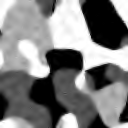
\includegraphics[width=0.32\linewidth]{compressive-sampling/geometrical/geometrical-wavelets.png} &
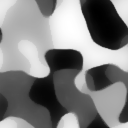
\includegraphics[width=0.32\linewidth]{compressive-sampling/geometrical/geometrical-manifold.png}\\
Original $f$  & Wavelets, SNR=25.7dB & Manifold, SNR=31.3dB
\end{tabular}
}{
Compressive sensing reconstruction results on a geometrical image with sparsity prior in wavelets and with the manifold model of affine edges.
The number of sensed vectors is $n_0 = n/8$ where $n$ is the number of pixels. %
}{fig-geometrical-cs}


%%%%%%%%%%%%%%%%%%%%%%%%%%%%%%%%%%%%%%%%%%%%%%%%%%%%%%%%%%%%%%
\myparagraph{Locally parallel textures.}
Figure \ref{fig-fingerprint-inpaint} shows an example of inpainting of a fingerprint image using the manifold of 2D oscillations \eqref{eq-defn-oscillations-2d}. Figure \ref{fig-fig-fingerprint-cs} shows the compressive sensing reconstruction from the same image, where the manifold prior is compared to a sparsity prior \eqref{eq-defn-sparsity-prior} in a local Gabor redundant frame, see \cite{mallat-book}. Such local oscillating atoms have been introduced with success for texture decomposition and inpainting in \cite{starck-inpainting,fadili-inpainting-cj}. The manifold prior is better able to capture the geometric regularity of the texture than the sparsity prior that diffuses the orientation information over several Gabor coefficients.

\myfigure{
\begin{tabular}{c@{\hspace{1mm}}c@{\hspace{1mm}}c@{\hspace{1mm}}c}
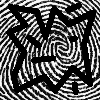
\includegraphics[width=0.24\linewidth]{locpar-inpainting/fingerprint3-iter1.png} &
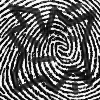
\includegraphics[width=0.24\linewidth]{locpar-inpainting/fingerprint3-iter2.png} &
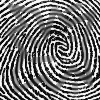
\includegraphics[width=0.24\linewidth]{locpar-inpainting/fingerprint3-iter5.png} &
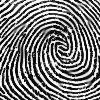
\includegraphics[width=0.24\linewidth]{locpar-inpainting/fingerprint3-final.png} \\
Iter. \#1 & Iter. \#2 & Iter. \#3 & Iter. \#50
\end{tabular}
}{
Iterations of the inpainting reconstruction algorithm on a 
locally parallel texture. %
}{fig-fingerprint-inpaint}


\myfigure{
\begin{tabular}{c@{\hspace{2mm}}c@{\hspace{2mm}}c}
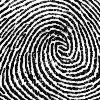
\includegraphics[width=0.32\linewidth]{locpar-cs/fingerprint3-original.png}&
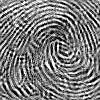
\includegraphics[width=0.32\linewidth]{locpar-cs/fingerprint3-spars.png}&
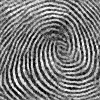
\includegraphics[width=0.32\linewidth]{locpar-cs/fingerprint3-manifold.png}\\
Original $f$  & 
Gabor, SNR=7.9dB & 
Manifold, SNR=9.5dB
\end{tabular}
}{
Compressive sensing reconstruction results on a locally parallel texture with sparsity prior in a redundant Gabor dictionary and with the manifold model. The number of sensed vectors is $n_0 = n/4$ where $n$ is the number of pixels. %
}{fig-fig-fingerprint-cs}


%%%%%%%%%%%%%%%%%%%%%%%%%%%%%%%%%%%%%%%%%%%%%%%%%%%%%%%%%%%%%%
\myparagraph{Sparse patches.}
Figure \ref{fig-reptilskin-cs} shows a reconstruction from compressive sensing using a manifold prior in the sparse texture ensemble \eqref{eq-sparsity-texture}. The dictionary $D$ is learned by minimizing $E_{\Mm_{D}}(f_e)$ for an exemplar texture $f_e$ that is close to the texture $f$ to recover. In practice, both image are extracted from different localization of the same image. The central part of the texture is badly reconstructed, because this part is not similar to the exemplar $f_e$. % In this central area, patches of the texture $f$ are too far away from the manifold model $\Mm$.

\myfigure{
\begin{tabular}{c@{\hspace{2mm}}c@{\hspace{2mm}}c@{\hspace{2mm}}c}
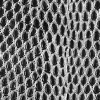
\includegraphics[width=0.24\linewidth]{compressive-sampling/reptilskin/reptilskin-original.png} &
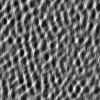
\includegraphics[width=0.24\linewidth]{compressive-sampling/reptilskin/reptilskin-iter-001.png} &
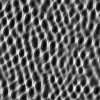
\includegraphics[width=0.24\linewidth]{compressive-sampling/reptilskin/reptilskin-iter-002.png} &
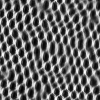
\includegraphics[width=0.24\linewidth]{compressive-sampling/reptilskin/reptilskin-iter-010.png}\\
Original $f$  & Iter. \#1 & Iter. \#1 & Iter. \#20
\end{tabular}
}{
Iterations of compressive sensing reconstruction results using a manifold model in a learned dictionary.
The number of sensed vectors is $n_0 = n/6$ where $n$ is the number of pixels. %
}{fig-reptilskin-cs}

Figure \ref{fig-corral-inpainting} shows a comparison of inpainting with a sparse prior \eqref{eq-defn-sparsity-prior}  in a translation invariant wavelet frame and a sparse patch manifold model prior. The dictionary $D$ is learned from a set of patches $p_{x_i}(y)$ extracted from the observed data, where the point $x_i$ are located at a distance larger than $\tau$ from the missing region to be inpainted. The resulting algorithm is similar to the inpainting algorithm of Mairal et al. \cite{mairal-color}, although they use a more complicated scheme to learn a dictionary with missing data. 

\myfigure{
\begin{tabular}{c@{\hspace{2mm}}c@{\hspace{2mm}}c@{\hspace{2mm}}c}
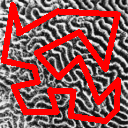
\includegraphics[width=0.32\linewidth]{inpainting/corral/corral-mask.png} &
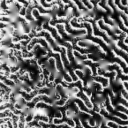
\includegraphics[width=0.32\linewidth]{inpainting/corral/corral-wavelets.png}&
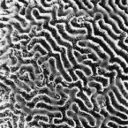
\includegraphics[width=0.32\linewidth]{inpainting/corral/corral-manifold.png}\\
Measurements $y$ & Wavelets, SNR=22.5dB & 
Manifold, SNR=31.1dB
\end{tabular}
}{
Comparison of inpainting using a sparsity prior in a wavelet basis and the sparse manifold model with a dictionary learned from the observed data $y$.
%
}{fig-corral-inpainting}




%%%%%%%%%%%%%%%%%%%%%%%%%%%%%%%%%%%%%%%%%%%%%%%%%%%%%%%%%%%%%%
%%%%%%%%%%%%%%%%%%%%%%%%%%%%%%%%%%%%%%%%%%%%%%%%%%%%%%%%%%%%%%
%%%%%%%%%%%%%%%%%%%%%%%%%%%%%%%%%%%%%%%%%%%%%%%%%%%%%%%%%%%%%%
\section*{Conclusion}

This paper has reviewed several manifold models for sounds, images and textures. These models constrain the set of patches extracted from the image and  describe efficiently the non-linear geometry of some classes of natural signals and images. A new manifold pursuit algorithm is used to regularize ill-posed inverse problem while maintaining the manifold model constraints. Results on various images and textures show how this manifold-driven restoration enhances variational models based on sparse expansions for inpainting and compressive sensing reconstruction. 


%%%%%%%%%%%%%%%%%%%%%%%%%%%%%%%%%%%%%%%%%%%%%%%%%%%%%%%%%%%%%%
%%%%%%%%%%%%%%%%%%%%%%%%%%%%%%%%%%%%%%%%%%%%%%%%%%%%%%%%%%%%%%
%%%%%%%%%%%%%%%%%%%%%%%%%%%%%%%%%%%%%%%%%%%%%%%%%%%%%%%%%%%%%%
\section*{Acknowledgments}

I would like to thank the anonymous reviewers for their comments that helped to improve the quality of the manuscript. 


% \bibliographystyle{siam}  % plain alpha
\bibliographystyle{elsart-num}
\bibliography{bibliography}

\end{document}
